\documentclass[12pt,a4paper]{article}

\usepackage[brazil]{babel}
\usepackage[utf8]{inputenc}
\usepackage[T1]{fontenc}
\usepackage{listings}

\usepackage{lmodern}

\usepackage{geometry}
\geometry{margin=2.5cm}

\usepackage{graphicx}
\usepackage{float}
\usepackage{amsmath}
\usepackage{amssymb}

\usepackage{booktabs}
\usepackage{caption}
\usepackage{subcaption}

\usepackage{hyperref}
\hypersetup{
    colorlinks=true,
    linkcolor=black,
    citecolor=black,
    urlcolor=black
}

% -------------------------------------------------
% Informações do trabalho
% -------------------------------------------------
\title{
    \textbf{Exploração e Análise de Dados por Técnicas de Aprendizado Não-Supervisionado}\\
    \vspace{0.3cm}
    \large IMD3003 – Aprendizado de Máquina Não-Supervisionado
}

\author{
    Gil César Faria
}

\date{15 de Dezembro de 2025}

% -------------------------------------------------
\begin{document}
\maketitle

% -------------------------------------------------
\section{Introdução}

O crescimento contínuo de sistemas de software complexos, especialmente no contexto de integrações e arquiteturas distribuídas, tem gerado grandes volumes de artefatos técnicos cuja análise manual se torna cada vez mais custosa. Em cenários reais, como projetos de integração baseados em Apache Camel, diferentes rotas podem compartilhar padrões arquiteturais e funcionais semelhantes, ainda que apresentem variações sintáticas ou implementações específicas. Identificar esses padrões de forma sistemática é um desafio relevante, especialmente na ausência de rótulos previamente definidos.

Neste contexto, técnicas de Aprendizado de Máquina Não-Supervisionado tornam-se uma alternativa adequada para explorar estruturas latentes nos dados, permitindo a identificação de agrupamentos naturais sem a necessidade de conhecimento prévio sobre as classes. Em particular, métodos de clusterização possibilitam agrupar instâncias com características semelhantes, enquanto técnicas de redução de dimensionalidade auxiliam na visualização e interpretação desses agrupamentos em espaços de menor dimensão.

Este trabalho investiga a aplicação de técnicas de aprendizado não-supervisionado para a análise e agrupamento de rotas Apache Camel, a partir de representações semânticas derivadas automaticamente do código-fonte. Inicialmente, cada rota é descrita por um conjunto de atributos semânticos que capturam aspectos arquiteturais e funcionais relevantes. Em seguida, são aplicados algoritmos de clusterização para identificar grupos de rotas com comportamento semelhante, bem como técnicas de projeção para apoiar a análise visual dos resultados.

O objetivo principal do trabalho é avaliar a capacidade dessas técnicas em revelar padrões arquiteturais recorrentes, contribuindo para a compreensão do sistema analisado e apoiando atividades como documentação, refatoração e evolução arquitetural. Além disso, o estudo busca discutir as vantagens e limitações das abordagens empregadas, considerando o impacto das escolhas de pré-processamento, parâmetros e algoritmos utilizados.

O restante deste relatório está organizado da seguinte forma: a Seção~2 descreve o conjunto de dados e suas principais características; a Seção~3 detalha as etapas de pré-processamento realizadas; a Seção~4 apresenta as técnicas de aprendizado não-supervisionado aplicadas; a Seção~5 discute os resultados obtidos e as visualizações geradas; e, por fim, a Seção~6 apresenta as conclusões do trabalho.

% -------------------------------------------------
\section{Descrição do Conjunto de Dados}

O conjunto de dados utilizado neste trabalho é composto por rotas de integração implementadas com o framework Apache Camel que utilizam linguagem de programação Java, extraídas de um sistema real de software voltado à integração entre serviços e sistemas heterogêneos. Cada rota representa um fluxo de processamento responsável por orquestrar chamadas a componentes internos e externos, incluindo serviços REST, serviços SOAP, mensageria e sistemas legados.

As rotas foram inicialmente coletadas a partir do código-fonte do projeto, considerando-se apenas aquelas efetivamente utilizadas em produção. Como as rotas não possuem rótulos predefinidos que indiquem seu papel arquitetural ou funcional, o problema abordado neste trabalho caracteriza-se naturalmente como uma tarefa de aprendizado não-supervisionado.

Para viabilizar a aplicação das técnicas de aprendizado de máquina, cada rota foi convertida em uma representação semântica estruturada. Essa representação é derivada automaticamente do código-fonte da rota e descreve aspectos arquiteturais e funcionais relevantes, tais como padrões de integração utilizados, componentes Camel empregados, tipos de endpoints acessados, estratégias de tratamento de erros e características gerais do fluxo de processamento. Dessa forma, o conjunto de dados final não é composto pelo código-fonte em si, mas por descrições semânticas que capturam a intenção e o comportamento de cada rota.

O conjunto de dados contém 1734 classes java correspondentes às rotas analisadas, todas descritas por um conjunto homogêneo de atributos semânticos. Esses atributos são majoritariamente categóricos ou textuais, refletindo a natureza qualitativa das decisões arquiteturais presentes nas rotas. Não há informações de classe ou rótulos associados às instâncias, reforçando o caráter exploratório da análise realizada.

A escolha desse conjunto de dados justifica-se por representar um cenário realista e complexo, no qual a identificação manual de padrões arquiteturais é difícil e suscetível a subjetividade. Além disso, o domínio de integração de sistemas apresenta alta variabilidade estrutural, tornando-o adequado para a avaliação do potencial de técnicas de clusterização e redução de dimensionalidade na descoberta de estruturas latentes nos dados.

% -------------------------------------------------
\section{Pré-processamento dos Dados}

O pré-processamento dos dados teve como objetivo transformar rotas Apache Camel, originalmente descritas em código-fonte Java DSL, em representações estruturadas e semanticamente comparáveis, adequadas para a aplicação de técnicas de aprendizado não-supervisionado. Como o código Java apresenta elevada variabilidade sintática e detalhes específicos de implementação, foi necessária uma etapa de abstração que priorizasse aspectos arquiteturais e funcionais relevantes das rotas.

Essa abstração foi realizada por meio da geração automática de descrições semânticas estruturadas utilizando um modelo de linguagem de grande porte (LLM), executado localmente via o runtime Ollama. O modelo utilizado foi o \textit{Qwen 2.5} com 7 bilhões de parâmetros, invocado individualmente para cada rota. A execução local do modelo permitiu controle total sobre o processo, além de reprodutibilidade e independência de serviços externos.

Para cada rota, o código Java DSL é fornecido integralmente ao modelo por meio de um prompt especializado, que instrui explicitamente a geração de uma representação conceitual em formato JSON. Esse prompt direciona o modelo a descrever a intenção arquitetural da rota, ignorando detalhes sintáticos, e a identificar padrões de integração, componentes utilizados, fluxo lógico de execução e estratégias de tratamento de exceções.

% =========================================================
% QUADRO DO PROMPT – DESCRIÇÃO SEMÂNTICA DAS ROTAS
% (alinhamento total à esquerda)
% =========================================================

\lstdefinestyle{promptbox}{
  basicstyle=\ttfamily\footnotesize,
  columns=fullflexible,
  breaklines=true,
  breakatwhitespace=false,
  breakindent=0pt,
  frame=single,
  framerule=0.4pt,
  xleftmargin=0.6em,
  xrightmargin=0.6em,
  aboveskip=0pt,
  belowskip=0pt,
  literate=
    {á}{{\'a}}1 {à}{{\`a}}1 {ã}{{\~a}}1 {â}{{\^a}}1
    {é}{{\'e}}1 {ê}{{\^e}}1
    {í}{{\'i}}1
    {ó}{{\'o}}1 {ô}{{\^o}}1 {õ}{{\~o}}1
    {ú}{{\'u}}1
    {ç}{{\c{c}}}1
    {Á}{{\'A}}1 {À}{{\`A}}1 {Ã}{{\~A}}1 {Â}{{\^A}}1
    {É}{{\'E}}1 {Ê}{{\^E}}1
    {Í}{{\'I}}1
    {Ó}{{\'O}}1 {Ô}{{\^O}}1 {Õ}{{\~O}}1
    {Ú}{{\'U}}1
    {Ç}{{\c{C}}}1
}

\vspace{0.6\baselineskip}

\begin{figure}[H]
\centering
\begin{minipage}{0.97\textwidth}
\lstset{style=promptbox}
\begin{lstlisting}
Analise a rota Apache Camel descrita em Java DSL a seguir e gere uma DESCRIÇÃO SEMÂNTICA ESTRUTURADA da rota.

O objetivo é capturar a INTENÇÃO ARQUITETURAL e FUNCIONAL da rota, e NÃO sua sintaxe ou detalhes de implementação.

Gere a saída estritamente no seguinte formato JSON:

{
  "route_id": "",
  "route_start": "",
  "components_used": [],
  "patterns_detected": [],
  "flow_summary": [],
  "transformations": [],
  "endpoints_called": [],
  "internal_beans": [],
  "error_handling": "",
  "fingerprint": ""
}

REGRAS:
- Responda SOMENTE o JSON, sem qualquer texto adicional.
- Utilize Português Brasileiro.
- Ignore detalhes sintáticos do Java DSL.
- Identifique padrões de integração (Enterprise Integration Patterns).
- Liste apenas componentes Apache Camel relevantes.
- Resuma o fluxo em passos conceituais de alto nível.
- Gere uma fingerprint curta que represente a sequência principal da rota.

Agora analise a rota abaixo:
{{CODIGO_FONTE}}
\end{lstlisting}
\end{minipage}
\caption{Prompt para geração da descrição semântica das rotas.}
\label{fig:prompt-descricao-semantica}
\end{figure}

O resultado dessa etapa é uma descrição semântica estruturada em JSON, composta por um conjunto fixo de campos homogêneos para todas as rotas. Entre os atributos extraídos estão o identificador da rota, o ponto de entrada, os componentes Apache Camel utilizados, os padrões de integração detectados, os endpoints externos acessados, os beans internos invocados, uma descrição conceitual do fluxo em etapas de alto nível, as transformações aplicadas e a forma como exceções são tratadas. Adicionalmente, é gerada uma \emph{fingerprint} textual curta que resume a sequência principal de processamento da rota.

Como etapa adicional de validação, todas as descrições semânticas geradas foram submetidas a um processo automático de verificação de conformidade sintática. Cada arquivo JSON foi parseado utilizando o utilitário \textit{jq}, de modo a identificar descrições mal formadas. Os casos que apresentaram erro de parsing — totalizando 170 arquivos — foram analisados e corrigidos manualmente, garantindo que apenas representações JSON bem formadas fossem mantidas no conjunto de dados final.

Após essa etapa de limpeza e validação, as representações semânticas estruturadas são utilizadas diretamente como entrada para a geração de embeddings. A transformação para o espaço vetorial é realizada pelo modelo \textit{sentence-transformers/all-MiniLM-L6-v2}, empregado por meio da biblioteca SentenceTransformers, o qual projeta cada descrição textual em um vetor denso de 384 atributos. Esse modelo é treinado especificamente para capturar similaridades semânticas globais entre textos em um espaço contínuo, permitindo a comparação direta entre rotas a partir de suas descrições conceituais. O resultado desse processo é armazenado em um arquivo \texttt{embeddings.csv}, cuja estrutura é composta pelos seguintes campos:

\begin{itemize}
  \item \texttt{route\_id}: identificador único da rota Apache Camel.
  \item \texttt{path}: caminho do arquivo fonte da rota no repositório.
  \item \texttt{embedding}: vetor denso de 384 dimensões que representa semanticamente a rota.
  \item \texttt{error}: campo utilizado durante a validação para sinalizar descrições JSON mal formadas.
\end{itemize}

No conjunto final de dados, a coluna \texttt{error} encontra-se vazia, uma vez que todos os arquivos JSON inicialmente inválidos foram identificados por meio de verificação automática e corrigidos manualmente antes da geração definitiva dos embeddings. Como resultado, o pré-processamento produz um conjunto de instâncias semanticamente consistentes e representadas em um espaço vetorial de dimensão fixa, adequado para a aplicação de algoritmos de clusterização e técnicas de redução de dimensionalidade.

A Figura~\ref{fig:preprocessamento-pipeline} apresenta uma visão esquemática do pipeline de pré-processamento adotado neste trabalho. O processo inicia-se a partir do código-fonte das rotas Apache Camel, implementadas em Java DSL, que é fornecido como entrada para um modelo de linguagem responsável pela extração de descrições semânticas estruturadas. Essas descrições são geradas em formato JSON e capturam aspectos arquiteturais e funcionais das rotas, abstraindo detalhes sintáticos. Em seguida, as representações semânticas são transformadas em vetores densos por meio de um modelo de geração de embeddings, resultando em representações numéricas de dimensão fixa. Esse pipeline estabelece a base para as etapas subsequentes de clusterização e redução de dimensionalidade, permitindo a análise de similaridade entre rotas em um espaço vetorial contínuo.

\begin{figure}[H]
\centering
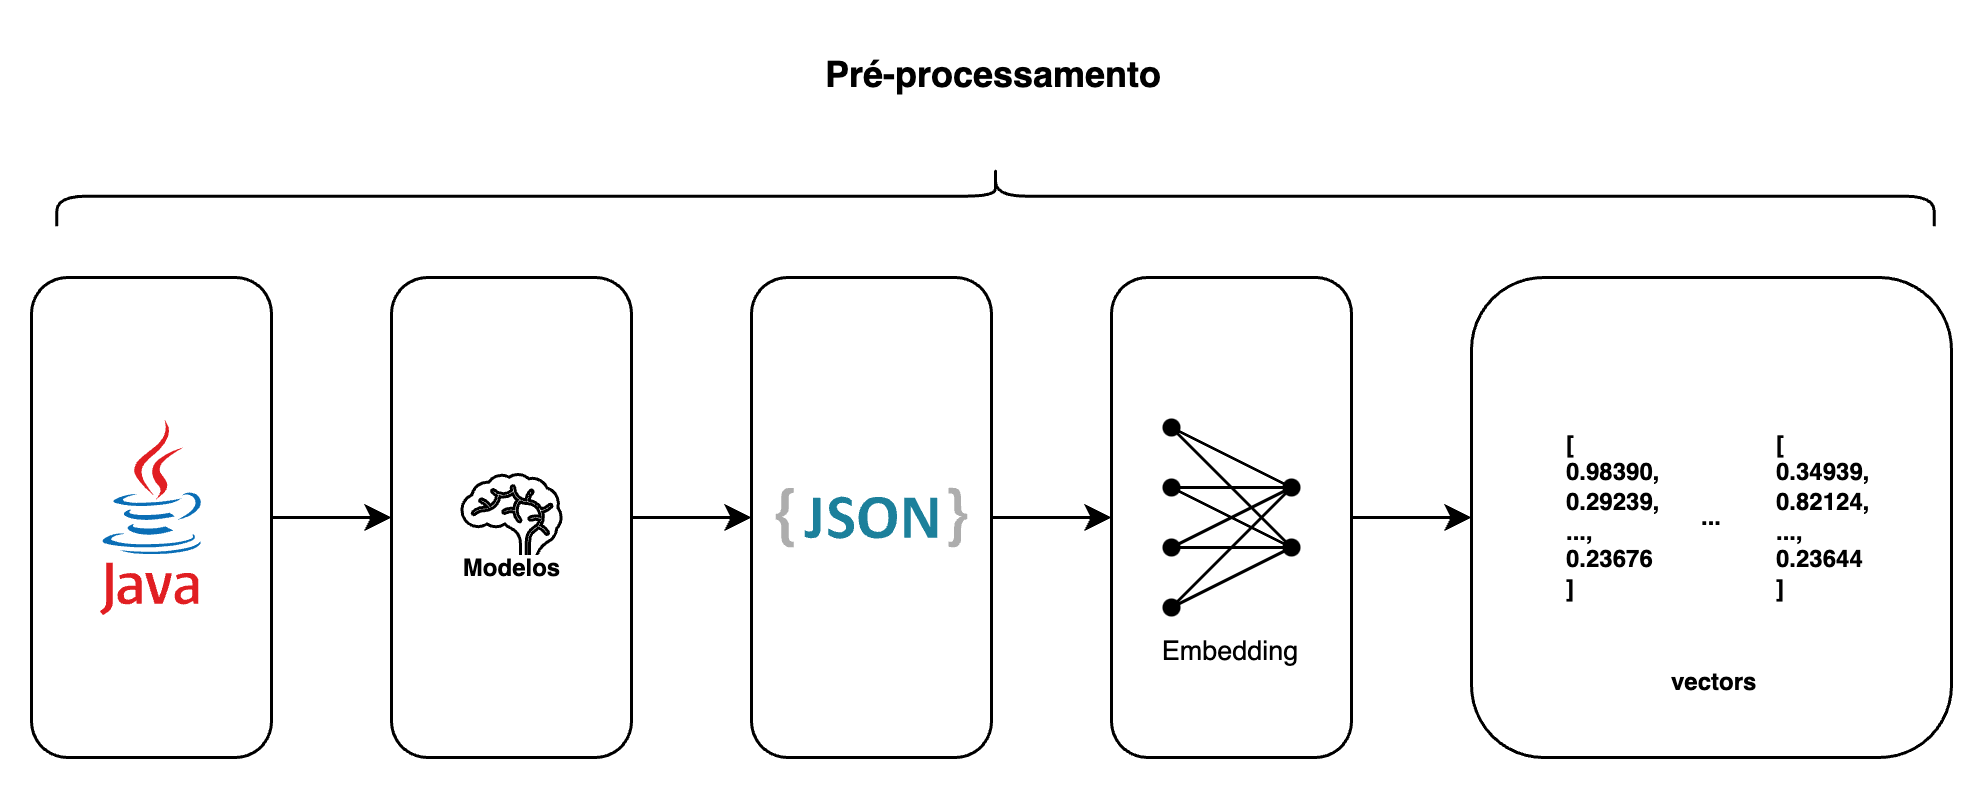
\includegraphics[width=\textwidth]{metodologia-imd3003-preprocessamento.png}
\caption{Pipeline de pré-processamento adotado, desde o código-fonte das rotas Apache Camel até a geração de vetores de embeddings.}
\label{fig:preprocessamento-pipeline}
\end{figure}

% -------------------------------------------------
\section{Técnicas de Aprendizado Não-Supervisionado}

A abordagem adotada neste trabalho seguiu um fluxo incremental no qual técnicas de redução de dimensionalidade foram aplicadas previamente à etapa de clusterização, com o objetivo de viabilizar tanto a visualização quanto a análise da estrutura dos dados. A clusterização foi realizada exclusivamente sobre projeções de menor dimensionalidade, obtidas a partir de embeddings normalizados, uma vez que a aplicação direta de algoritmos de agrupamento no espaço original de alta dimensão dificulta a interpretação dos resultados.

De forma geral, diferentes técnicas de redução de dimensionalidade foram exploradas de maneira independente, seguidas pela aplicação de algoritmos de clusterização sobre as projeções resultantes. Para cada combinação de método de redução e algoritmo de agrupamento, métricas de similaridade e parâmetros foram definidos por meio de buscas em grade (\textit{grid search}), permitindo avaliar sistematicamente o impacto dessas escolhas na estrutura dos agrupamentos obtidos. Todos os experimentos operaram sobre vetores densos de dimensão 384, gerados pelo modelo \textit{sentence-transformers/all-MiniLM-L6-v2} e normalizados individualmente por meio da norma L2.

A Figura~\ref{fig:etapas-ml} sintetiza o fluxo experimental adotado, ilustrando os diferentes caminhos explorados a partir dos embeddings normalizados, incluindo PCA e t-SNE em duas dimensões e UMAP em duas e três dimensões, bem como os algoritmos de clusterização aplicados em cada caso. Essa visão geral serve como referência para a descrição detalhada de cada experimento nas subseções a seguir.

\begin{figure}[H]
\centering
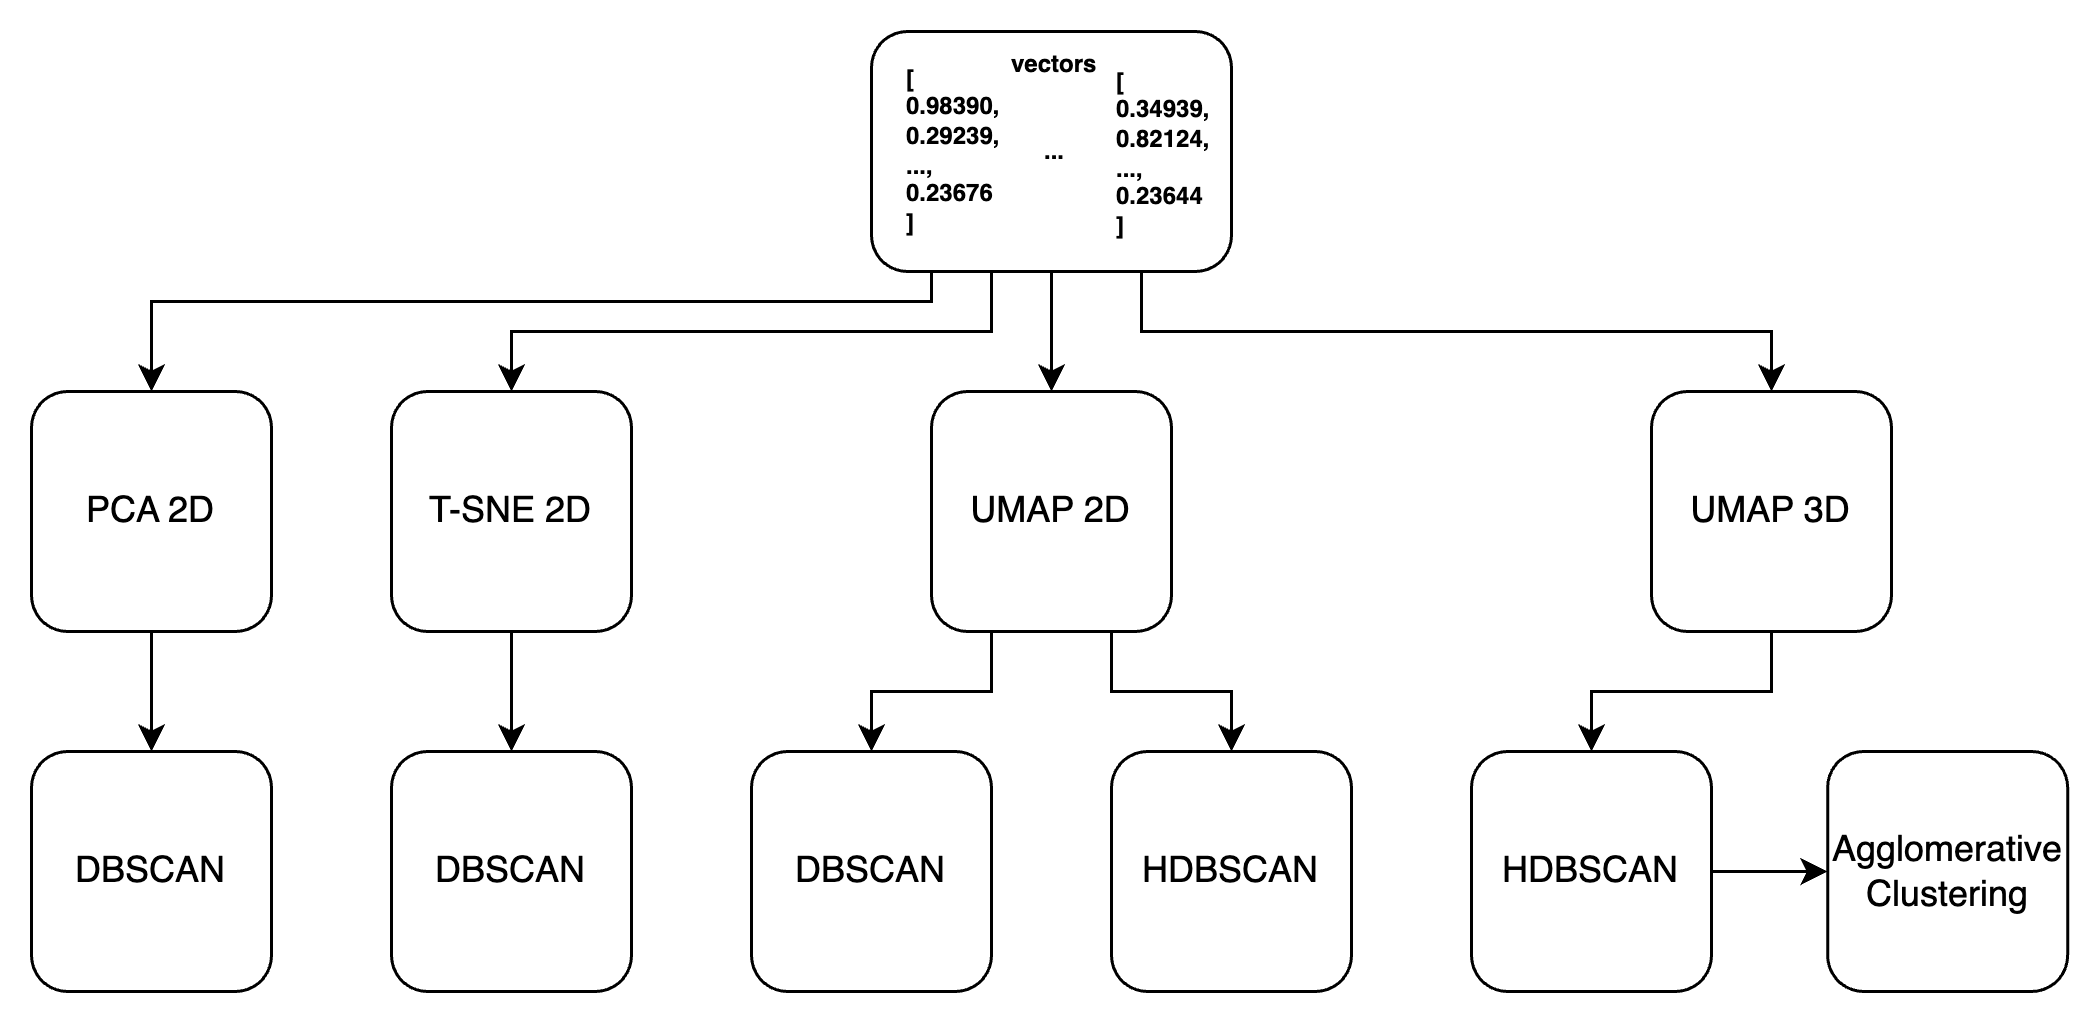
\includegraphics[width=\textwidth]{metodologia-imd3003-etapas-ML.png}
\caption{Fluxo das etapas aplicadas aos embeddings normalizados.}
\label{fig:etapas-ml}
\end{figure}

\subsection{PCA}

A Análise de Componentes Principais (PCA) foi utilizada como primeira técnica de redução de dimensionalidade com o objetivo de investigar a estrutura global dos embeddings gerados a partir das descrições semânticas das rotas. Por se tratar de um método linear, o PCA permite identificar direções de maior variância nos dados e serve como uma etapa inicial de diagnóstico, tanto para visualização quanto para avaliação da adequação de técnicas lineares ao problema em estudo.

O PCA foi aplicado sobre os embeddings normalizados de dimensão 384, utilizando a implementação disponível na biblioteca \textit{scikit-learn}. Foram consideradas duas configurações distintas: projeção em duas dimensões e projeção em três dimensões, ambas com \texttt{random\_state} fixado em 42 para garantir reprodutibilidade. Em ambos os casos, o PCA foi utilizado exclusivamente como uma transformação de projeção, sem modificar os vetores originais empregados nas demais etapas do pipeline.

Para avaliar a qualidade das projeções geradas, foi calculada a métrica de \textit{trustworthiness}, comparando-se as relações de vizinhança no espaço original de alta dimensão com aquelas observadas nos espaços reduzidos. O cálculo foi realizado com \texttt{n\_neighbors = 10}, permitindo quantificar o grau de preservação da estrutura local dos dados após a redução dimensional. Essa avaliação forneceu um critério objetivo para analisar o impacto da projeção linear antes da aplicação de algoritmos de clusterização.

As projeções obtidas por PCA em duas e três dimensões foram analisadas visualmente por meio de gráficos de dispersão, com o objetivo de identificar possíveis agrupamentos naturais ou padrões globais. Em seguida, o algoritmo DBSCAN foi aplicado diretamente sobre essas projeções, utilizando parâmetros fixos definidos de forma exploratória. Essa etapa permitiu avaliar o comportamento de um método de clusterização baseado em densidade quando aplicado a projeções lineares dos embeddings.

A aplicação do DBSCAN sobre as projeções obtidas por PCA permitiu avaliar visualmente o
comportamento do algoritmo de clusterização quando operando sobre uma redução linear dos
embeddings. As Figuras~\ref{fig:pca2d-dbscan} e~\ref{fig:pca3d-dbscan} apresentam,
respectivamente, as projeções em duas e três dimensões já com os rótulos de cluster
atribuídos, permitindo uma comparação direta entre as duas representações.

\begin{figure}[H]
\centering
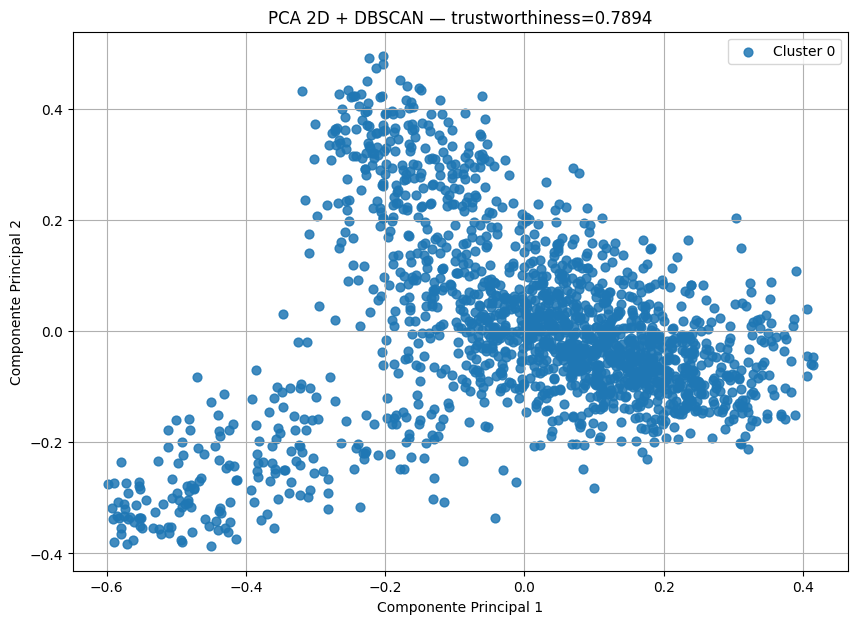
\includegraphics[width=0.85\textwidth]{pca2d-dbscan.png}
\caption{Projeção PCA em duas dimensões com aplicação do algoritmo DBSCAN sobre os embeddings normalizados. O valor de \textit{trustworthiness} indica preservação limitada da estrutura local após a redução linear.}
\label{fig:pca2d-dbscan}
\end{figure}
\begin{figure}[H]
\centering
\includegraphics[width=0.9\textwidth]{pca3d_dbscan.png}
\caption{Projeção PCA em três dimensões com aplicação do algoritmo DBSCAN sobre os embeddings normalizados. Apesar do aumento do valor de \textit{trustworthiness}, a projeção não resulta em uma separação clara entre agrupamentos, indicando limitações do PCA na captura da estrutura semântica dos dados.}
\label{fig:pca3d-dbscan}
\end{figure}


A análise combinada das métricas de preservação estrutural e dos resultados da clusterização indicou limitações do PCA para capturar adequadamente as relações semânticas presentes nos dados. Esses resultados motivaram a exploração de técnicas de redução de dimensionalidade não lineares, descritas nas subseções seguintes, com o objetivo de obter projeções mais adequadas à estrutura intrínseca dos embeddings.


\subsection{t-SNE}

O t-SNE foi empregado como técnica de redução de dimensionalidade não linear com o objetivo de capturar relações locais complexas entre os embeddings, não adequadamente representadas pelas projeções lineares obtidas com o PCA. Por preservar vizinhanças locais de forma probabilística, o método é particularmente adequado para revelar estruturas latentes em dados de alta dimensão, sendo utilizado neste trabalho como alternativa direta às limitações observadas nas projeções lineares.

Após aplicações exploratórias iniciais em duas dimensões, utilizadas para identificar uma região adequada no espaço de parâmetros, foi conduzida uma busca sistemática por hiperparâmetros por meio de \textit{grid search}. Foram avaliadas combinações de valores de \textit{perplexity} iguais a 10, 15 e 30, métodos de inicialização \texttt{random} e \texttt{pca}, taxas de aprendizado de 100, 200 e \texttt{auto}, valores de \textit{early exaggeration} de 8, 12 e 20, além do uso de uma etapa prévia de redução por PCA para 50 dimensões, mantida ativa em todas as configurações testadas.

A qualidade das projeções bidimensionais foi avaliada por meio da métrica de \textit{trustworthiness}, calculada com \texttt{n\_neighbors = 10}, comparando as relações de vizinhança no espaço original de 384 dimensões com aquelas observadas no espaço reduzido. A configuração de melhor desempenho foi selecionada com base no maior valor de trustworthiness observado, correspondendo aos parâmetros \textit{perplexity} igual a 30, inicialização baseada em PCA, taxa de aprendizado de 200, \textit{early exaggeration} igual a 20 e uso de redução prévia para 50 dimensões por PCA, resultando em um valor de trustworthiness de aproximadamente 0.956.

Sobre a projeção bidimensional obtida com essa configuração ótima, foi aplicado o algoritmo DBSCAN, permitindo identificar agrupamentos densos e semanticamente coerentes no espaço reduzido. A Figura~\ref{fig:tsne-dbscan} apresenta o resultado dessa combinação, evidenciando múltiplos clusters bem definidos, bem como a presença de um agrupamento dominante que concentra um número expressivo de instâncias, caracterizando um supercluster.

\begin{figure}[H]
\centering
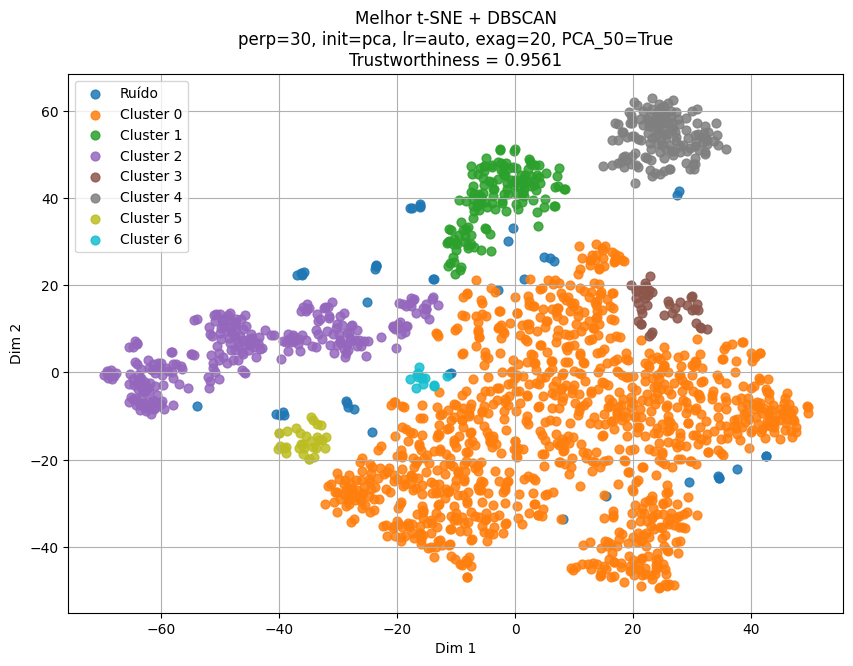
\includegraphics[width=0.9\textwidth]{tsne2d_dbscan.png}
\caption{Projeção t-SNE com aplicação do algoritmo DBSCAN sobre os embeddings normalizados, utilizando a configuração de melhor desempenho identificada no \textit{grid search}.}
\label{fig:tsne-dbscan}
\end{figure}

A presença desse supercluster sugere a existência de estruturas internas ou hierárquicas não plenamente capturadas na projeção bidimensional. Essa observação motivou a exploração do UMAP, com o objetivo de investigar de forma mais detalhada a organização interna desse agrupamento dominante e avaliar sua estabilidade sob diferentes configurações de redução de dimensionalidade.

\subsection{UMAP 2D}

O UMAP foi empregado como técnica de redução de dimensionalidade não linear para equilibrar a preservação de estruturas locais e globais, superando limitações observadas nas projeções obtidas com PCA e t-SNE. No contexto deste trabalho, o UMAP foi explorado principalmente para investigar de forma mais detalhada a organização interna dos agrupamentos, em especial o supercluster identificado nas projeções anteriores.

Foi realizada uma busca sistemática por hiperparâmetros por meio de \textit{grid search}. Foram avaliadas combinações dos parâmetros \textit{n\_neighbors} iguais a 5, 15, 30 e 50, e \textit{min\_dist} iguais a 0.0, 0.1 e 0.5, mantendo-se a métrica euclidiana. Para cada configuração, a qualidade da projeção foi avaliada por meio da métrica de \textit{trustworthiness}, calculada com \texttt{n\_neighbors = 10}.

Os resultados indicaram melhor desempenho para valores intermediários de \textit{n\_neighbors}, em particular 15, combinados com valores baixos de \textit{min\_dist}. A configuração selecionada apresentou \textit{n\_neighbors} igual a 15 e \textit{min\_dist} igual a 0.0, resultando em um valor de trustworthiness de aproximadamente 0.942, indicando preservação consistente das vizinhanças locais no espaço reduzido.

A aplicação do algoritmo DBSCAN sobre a projeção UMAP 2D obtida com essa configuração permitiu identificar agrupamentos compactos e bem separados, com redução significativa de ruído em comparação com as projeções baseadas em PCA e t-SNE, conforme ilustrado na Figura~\ref{fig:umap2d-dbscan}. No entanto, por assumir um parâmetro global de densidade, o DBSCAN ainda apresenta limitações na identificação de variações internas dentro de agrupamentos densos.

\begin{figure}[H]
\centering
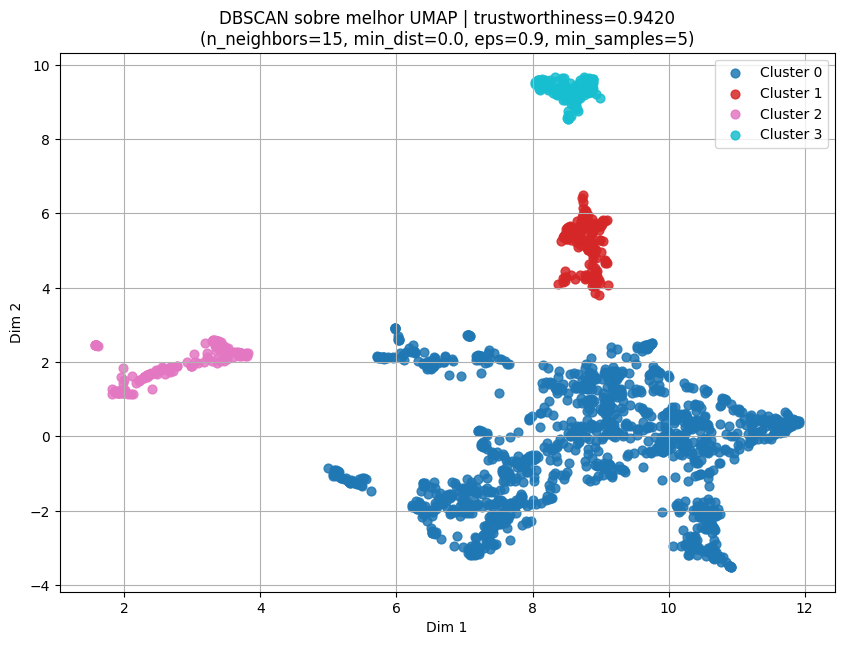
\includegraphics[width=0.9\textwidth]{umap2d_dbscan.png}
\caption{Projeção UMAP  com DBSCAN utilizando a configuração de melhor desempenho identificada no \textit{grid search}.}
\label{fig:umap2d-dbscan}
\end{figure}

Para contornar essa limitação, foi aplicado o algoritmo HDBSCAN sobre a mesma projeção UMAP 2D. O resultado, apresentado na Figura~\ref{fig:umap2d-hdbscan}, evidencia uma fragmentação mais detalhada do espaço projetado, revelando subestruturas internas previamente agrupadas pelo DBSCAN.

\begin{figure}[H]
\centering
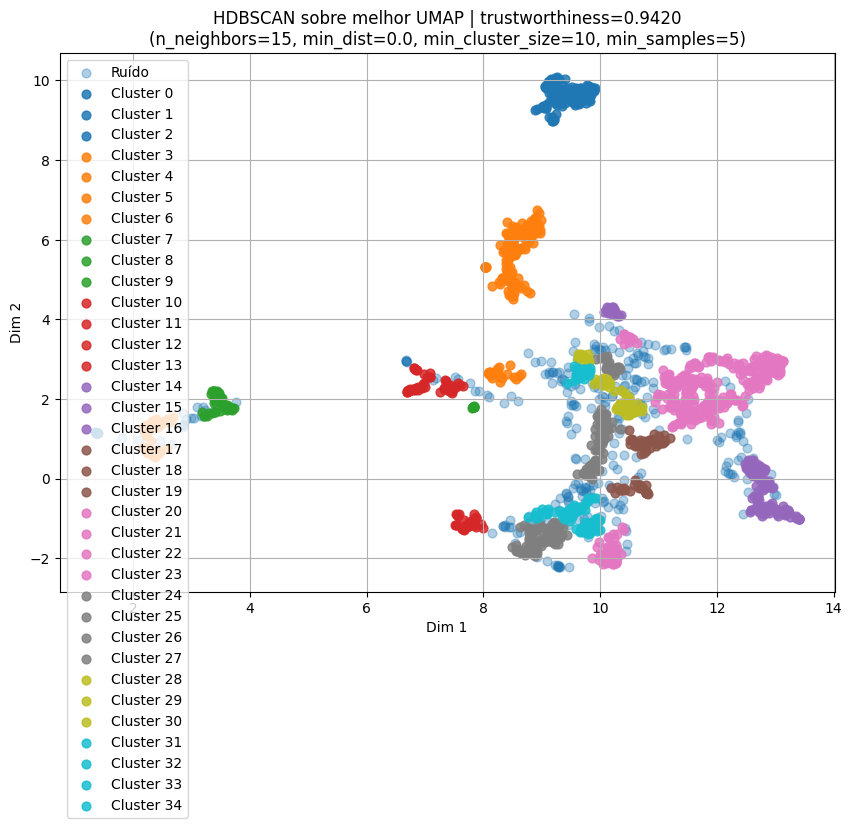
\includegraphics[width=0.9\textwidth]{umap2d_hdbscan.png}
\caption{Projeção UMAP com HDBSCAN evidenciando a identificação de múltiplos agrupamentos com diferentes densidades a partir da mesma configuração de redução dimensional.}
\label{fig:umap2d-hdbscan}
\end{figure}

Esse comportamento indica a presença de variações semânticas relevantes dentro de clusters densos e reforça a adequação do UMAP como técnica de redução de dimensionalidade para dados textuais complexos. Esses resultados motivaram a extensão da análise para projeções em três dimensões, discutidas na subseção seguinte.

\subsection{UMAP 3D}

Com o objetivo de investigar de forma mais aprofundada a organização estrutural dos agrupamentos identificados nas projeções bidimensionais, o UMAP foi estendido para uma projeção em três dimensões. A utilização de um espaço tridimensional permite maior expressividade geométrica, reduzindo sobreposições artificiais e facilitando a análise de estruturas hierárquicas que não se manifestam claramente em duas dimensões.

A projeção UMAP 3D foi obtida por meio de um \textit{grid search} refinado, no qual foram avaliadas combinações dos parâmetros \textit{n\_neighbors} iguais a 10, 15, 20 e 25, \textit{min\_dist} iguais a 0.0, 0.05, 0.10 e 0.20, utilizando a métrica de similaridade cosseno. Para cada configuração, a qualidade da projeção tridimensional foi avaliada por meio da métrica de \textit{trustworthiness}, calculada com \texttt{n\_neighbors = 10}, comparando as relações de vizinhança no espaço original de 384 dimensões com aquelas preservadas no espaço reduzido. A melhor configuração apresentou valor de trustworthiness de aproximadamente 0.954, indicando elevada preservação das estruturas locais após a redução dimensional.

Sobre a projeção UMAP 3D selecionada, foi inicialmente aplicado o algoritmo DBSCAN com o objetivo de identificar agrupamentos densos e regiões de ruído no espaço reduzido. A Figura~\ref{fig:umap3d-dbscan} apresenta o resultado dessa combinação, evidenciando a separação de estruturas globais, porém também mostrando que o supercluster identificado foi excessivamente fragmentado, inviabilizando o uso prático do resultado.

\begin{figure}[H]
\centering
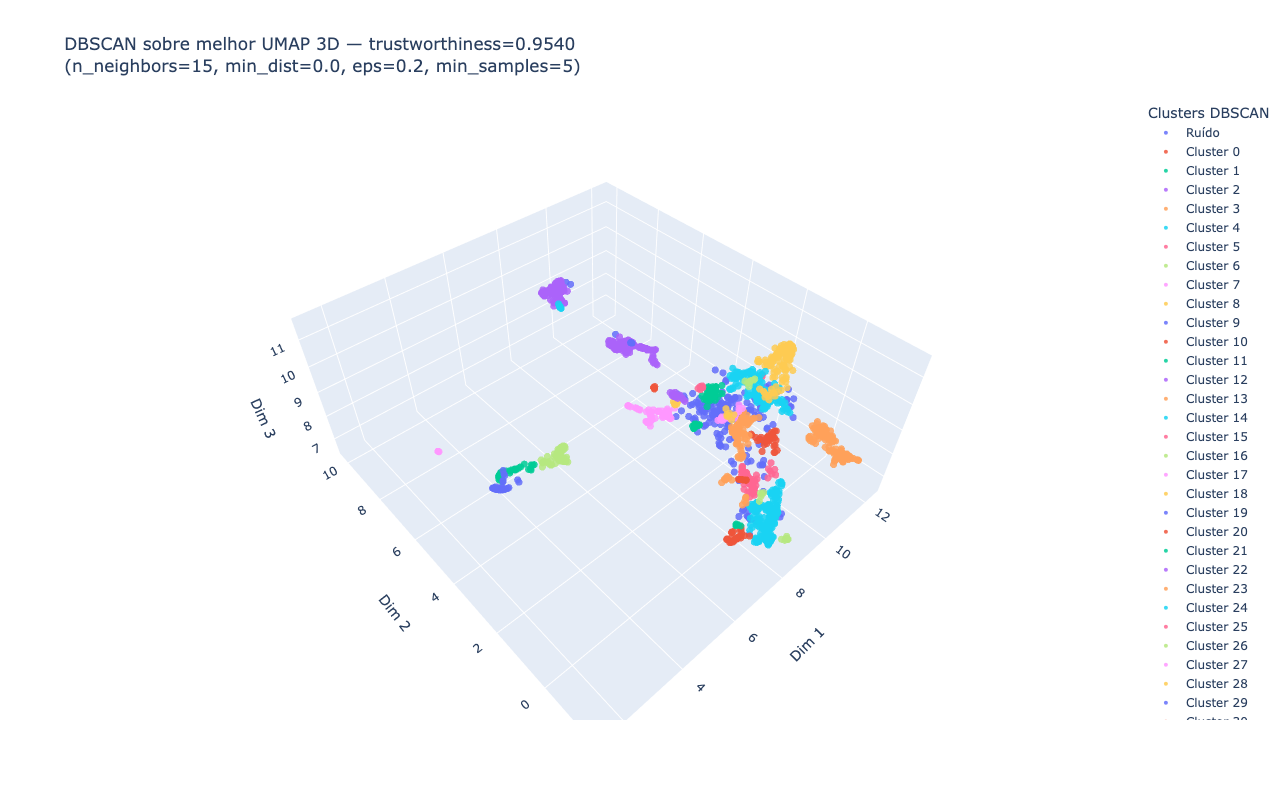
\includegraphics[width=0.9\textwidth]{umap3d_dbscan.png}
\caption{Projeção UMAP 3D com aplicação do algoritmo DBSCAN, evidenciando a fragmentação excessiva do supercluster.}
\label{fig:umap3d-dbscan}
\end{figure}

Com o objetivo de refinar a segmentação obtida pelo DBSCAN, foi aplicado o algoritmo HDBSCAN sobre a mesma projeção UMAP 3D, permitindo a identificação de agrupamentos com densidades variáveis. A Figura~\ref{fig:umap3d-hdbscan} apresenta o resultado dessa etapa, no qual observa-se uma segmentação mais equilibrada, com múltiplos clusters bem definidos e uma redução significativa da dependência de parâmetros globais de densidade, embora o supercluster ainda permaneça presente.

\begin{figure}[H]
\centering
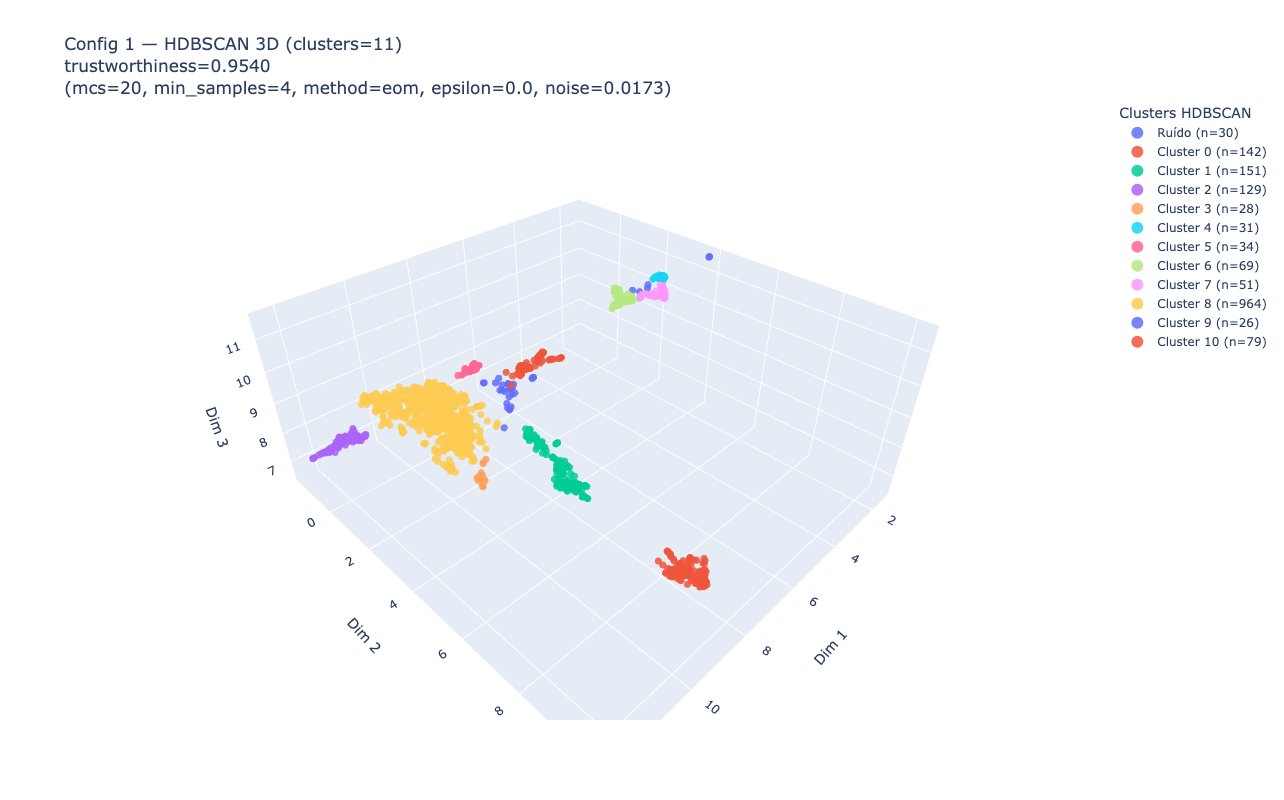
\includegraphics[width=0.9\textwidth]{umap3d_hdbscan.png}
\caption{Projeção UMAP 3D com aplicação do algoritmo HDBSCAN, apresentando melhor separação entre agrupamentos de densidades distintas, porém mantendo a presença de um supercluster dominante.}
\label{fig:umap3d-hdbscan}
\end{figure}

Para avaliar se o supercluster identificado poderia ser decomposto de forma significativa, foi realizada uma etapa adicional de clusterização restrita exclusivamente às instâncias pertencentes a esse agrupamento. Nessa etapa, foi conduzido um \textit{grid search} específico do algoritmo HDBSCAN, explorando diferentes combinações de \textit{min\_cluster\_size}, \textit{min\_samples}, método de seleção de clusters e valores de \textit{epsilon}. O objetivo foi verificar se ajustes finos nos parâmetros permitiriam revelar subestruturas semanticamente coerentes dentro do supercluster.

O melhor resultado obtido nesse processo é apresentado na Figura~\ref{fig:umap3d-supercluster-hdbscan}. Observa-se que, embora o algoritmo tenha identificado múltiplos agrupamentos, o resultado apresenta elevado nível de ruído e fragmentação excessiva, com a formação de diversos clusters de pequena cardinalidade. Em configurações alternativas avaliadas durante o \textit{grid search}, o comportamento foi igualmente insatisfatório, resultando predominantemente na manutenção de um único agrupamento dominante ou na geração de um número excessivo de clusters pouco interpretáveis.

\begin{figure}[H]
\centering
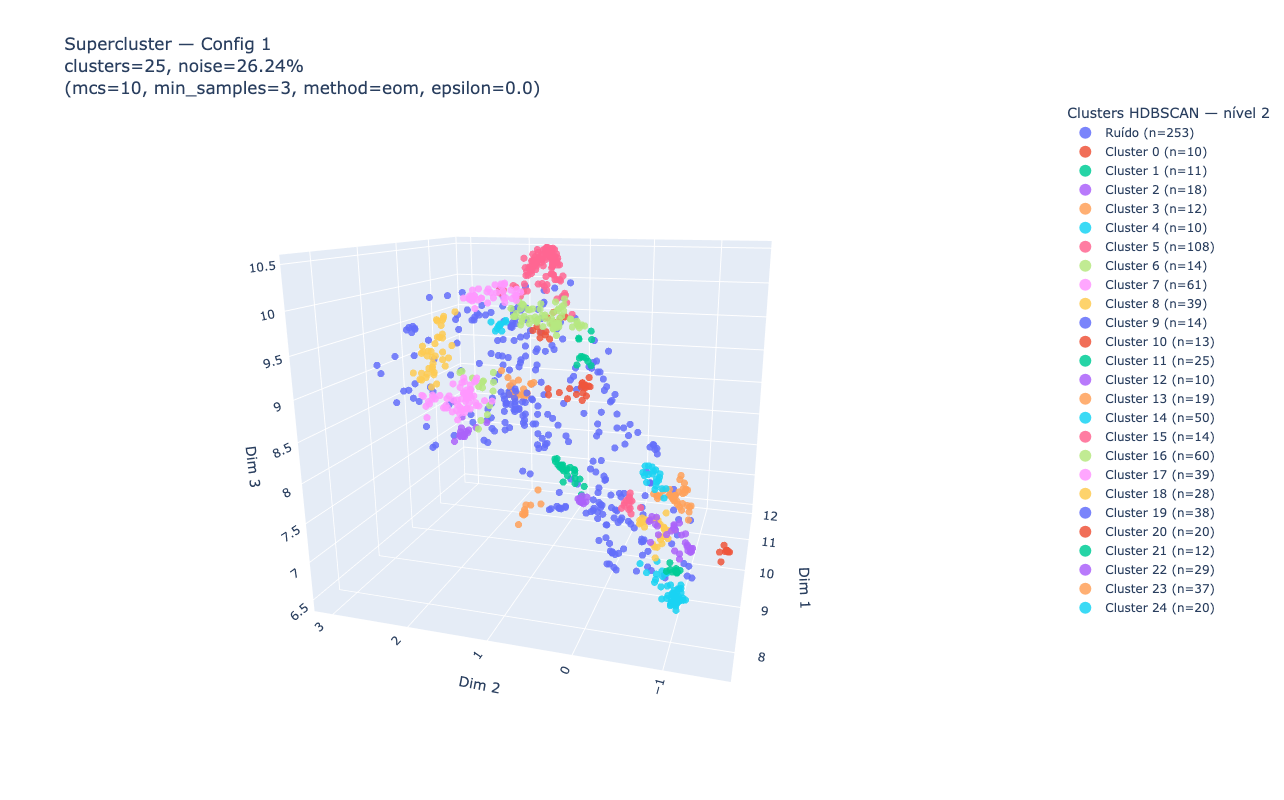
\includegraphics[width=0.9\textwidth]{umap3d_hdbscan_supercluster.png}
\caption{Resultado da aplicação do algoritmo HDBSCAN sobre o supercluster isolado na projeção UMAP 3D, evidenciando elevada fragmentação e presença significativa de ruído.}
\label{fig:umap3d-supercluster-hdbscan}
\end{figure}

Esses resultados indicam que, mesmo em um espaço tridimensional com elevada preservação das estruturas locais, o HDBSCAN não foi capaz de produzir uma decomposição estável e semanticamente interpretável do supercluster. Essa limitação motivou a adoção de uma abordagem alternativa baseada em clusterização hierárquica aglomerativa, a qual permite explorar explicitamente relações de similaridade globais e níveis hierárquicos de agrupamento sem depender de hipóteses locais de densidade.

A Figura~\ref{fig:umap3d-dendrogram} apresenta o dendrograma resultante da aplicação do algoritmo aglomerativo sobre o supercluster, utilizando o critério de ligação \textit{ward}. A análise visual do dendrograma permitiu identificar regiões de fusão mais estáveis e definir alturas de corte adequadas para a obtenção de um número reduzido de grupos semanticamente coerentes.

\begin{figure}[H]
\centering
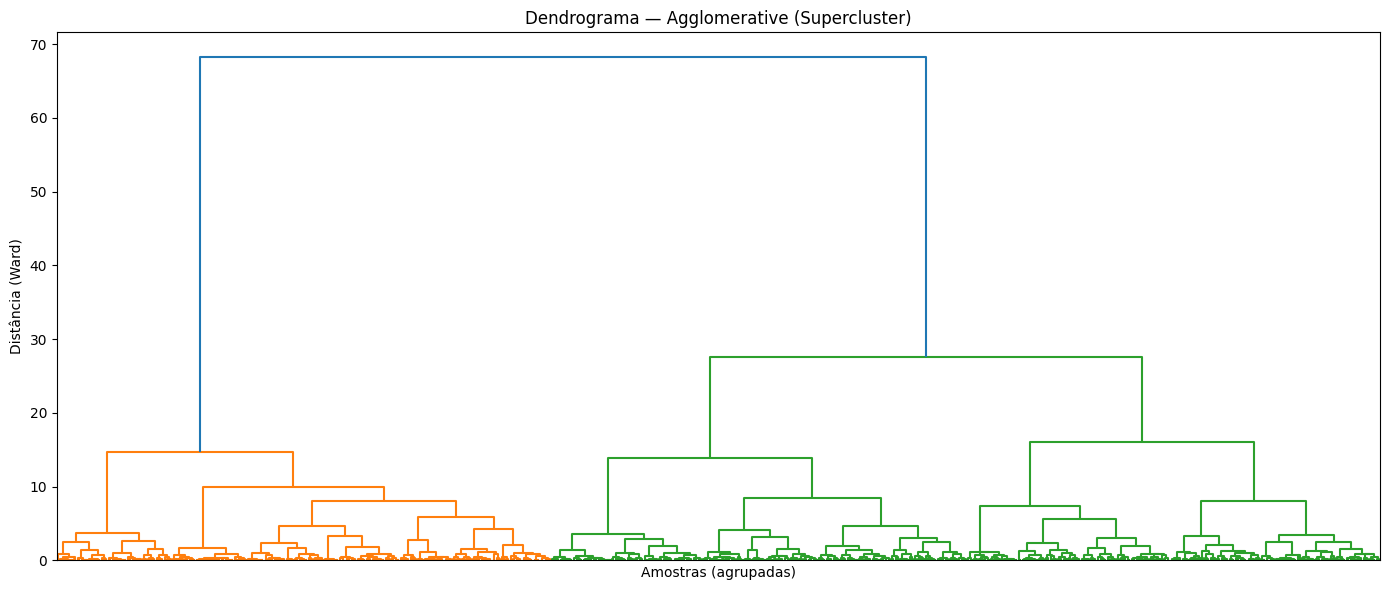
\includegraphics[width=1.05\textwidth]{umap3d_dendogram_supercluster.png}
\caption{Dendrograma obtido a partir da clusterização aglomerativa aplicada ao supercluster isolado na projeção UMAP 3D.}
\label{fig:umap3d-dendrogram}
\end{figure}

Com base nessa análise, foi selecionada uma altura de corte que resultou em um particionamento mais equilibrado do supercluster. A Figura~\ref{fig:umap3d-agglomerative} apresenta a abertura correspondente desse agrupamento, evidenciando subclusters mais estáveis e com melhor separação geométrica.

\begin{figure}[H]
\centering
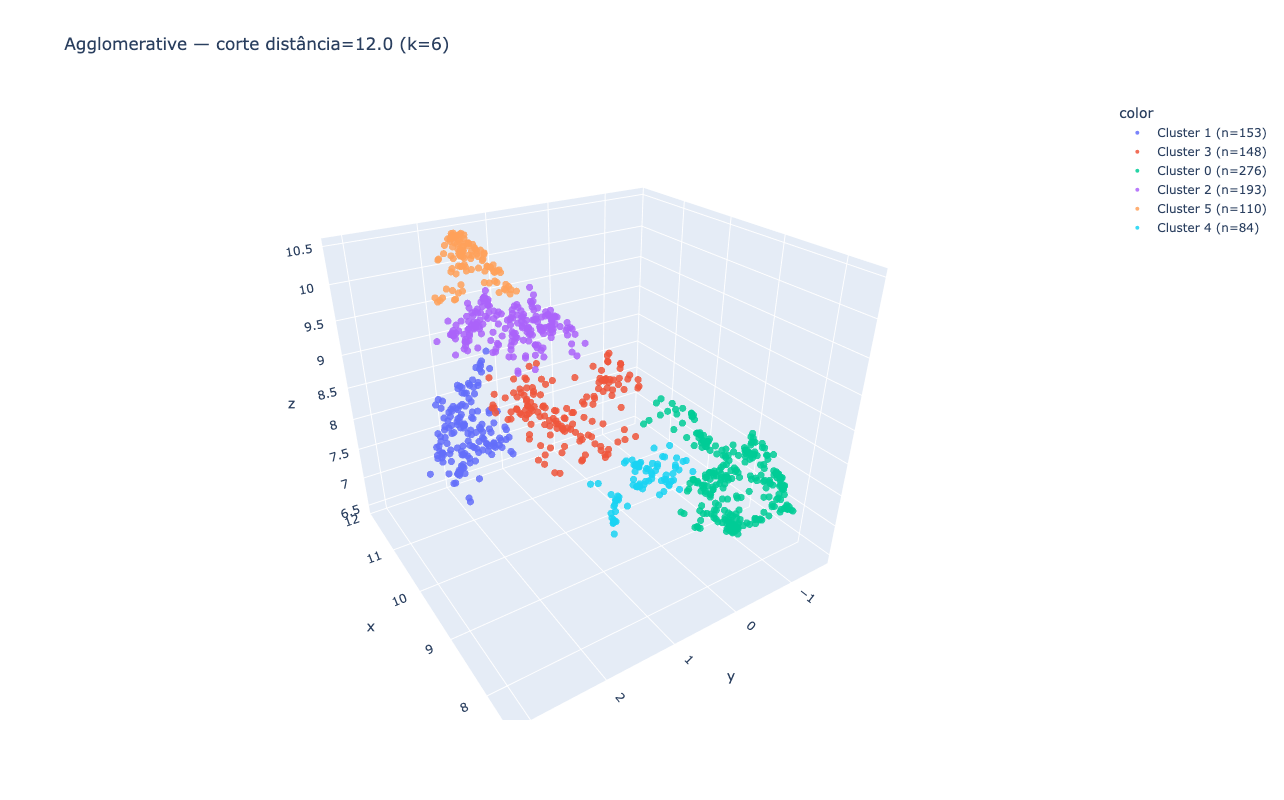
\includegraphics[width=1.1\textwidth]{umap3d_agglomerative_supercluster.png}
\caption{Resultado da clusterização aglomerativa aplicada ao supercluster, após definição do ponto de corte no dendrograma.}
\label{fig:umap3d-agglomerative}
\end{figure}

Por fim, os resultados foram recompostos em uma visão global de dois níveis, combinando os rótulos obtidos pelo HDBSCAN na projeção UMAP 3D com os subclusters derivados da clusterização aglomerativa aplicada ao supercluster. A Figura~\ref{fig:umap3d-final} apresenta essa recomposição final, permitindo visualizar simultaneamente a estrutura global dos agrupamentos e as variações semânticas internas previamente ocultas. Cabe destacar que a versão dos gráficos tridimensionais gerada no ambiente de notebooks Jupyter é interativa quando executada localmente em ferramentas como VS Code ou similares, possibilitando a rotação, aproximação e inspeção detalhada das estruturas dos clusters. Essa interatividade permite uma análise mais precisa das relações espaciais entre os agrupamentos e incentiva o leitor a explorar essas visualizações para um entendimento mais aprofundado, uma vez que a representação estática em 3D apresentada no documento possui limitações inerentes ao processo de projeção bidimensional em papel.


\begin{figure}[H]
\centering
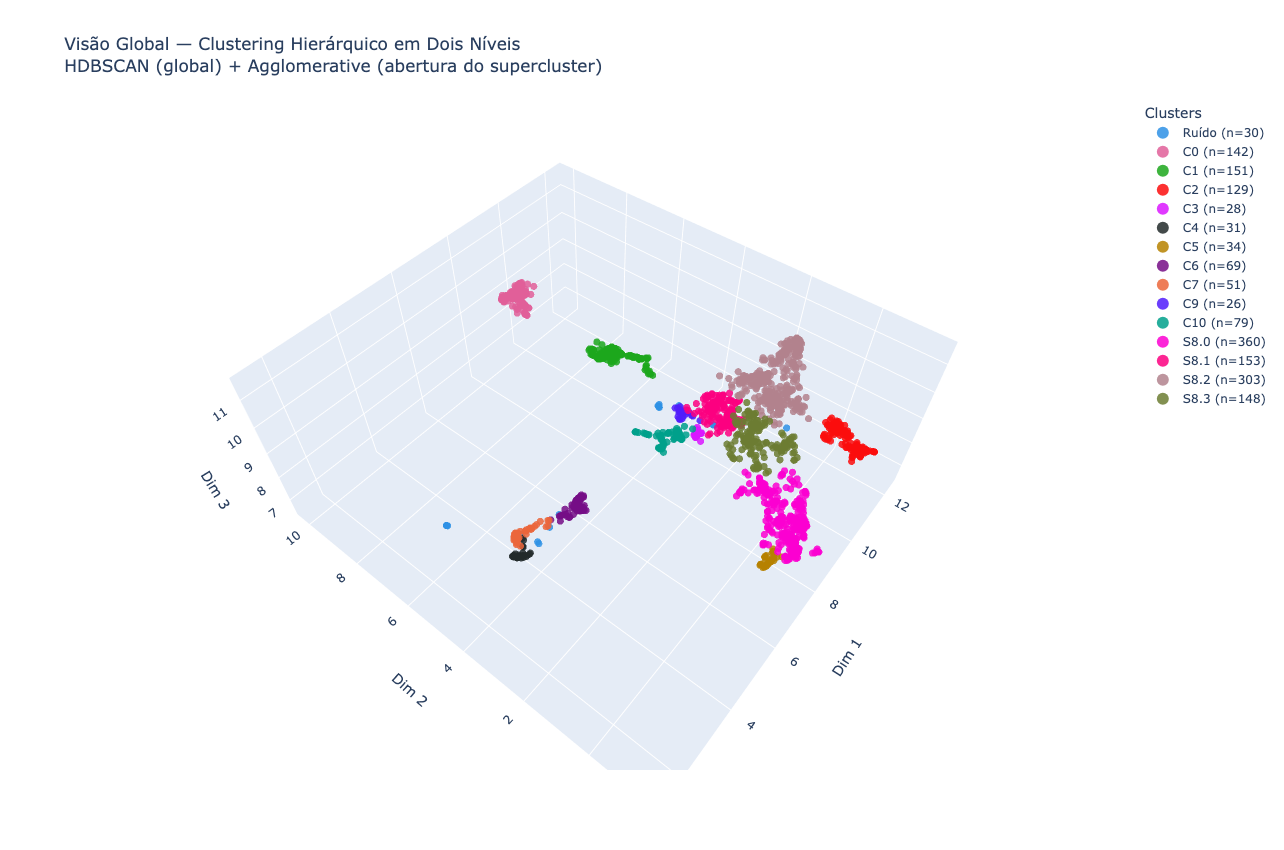
\includegraphics[width=1.1\textwidth]{umap3d_final.png}
\caption{Visão global recomposta da clusterização em dois níveis na projeção UMAP 3D, combinando HDBSCAN e clusterização aglomerativa.}
\label{fig:umap3d-final}
\end{figure}


\section{Análise e Interpretação dos Resultados}

Após a definição da clusterização final, baseada na combinação de HDBSCAN global com a abertura hierárquica do supercluster por meio de clusterização aglomerativa, procedeu-se à avaliação quantitativa da qualidade dos agrupamentos obtidos. Diferentemente das seções anteriores, cujo foco esteve na análise visual e estrutural das projeções, esta etapa concentra-se na interpretação de métricas objetivas de validação interna, calculadas diretamente sobre a projeção UMAP 3D e os rótulos finais dos clusters.

As métricas consideradas foram o coeficiente de Silhouette, o índice de Davies–Bouldin e o índice de Dunn. Em todas as avaliações, os pontos rotulados como ruído foram explicitamente removidos, de forma a evitar distorções na análise decorrentes de instâncias não atribuídas a clusters válidos.

\subsection{Coeficiente de Silhouette}

O coeficiente de Silhouette avalia simultaneamente a coesão interna dos clusters e a separação entre agrupamentos distintos, assumindo valores no intervalo $[-1,1]$, sendo valores mais elevados indicativos de melhor qualidade de clusterização. No presente trabalho, o coeficiente foi calculado sobre os vetores tridimensionais da projeção UMAP e os rótulos finais dos clusters, após a exclusão do ruído.

A Figura~\ref{fig:silhouette-final} apresenta o \textit{Silhouette Plot} da clusterização final. Observa-se que a média global do coeficiente, indicada pela linha tracejada, situa-se em um patamar positivo e consistente, sugerindo boa separação entre os clusters no espaço reduzido. Adicionalmente, nota-se que a maioria dos agrupamentos apresenta valores predominantemente positivos, embora com variações internas, refletindo diferenças naturais de densidade e coesão entre clusters globais e subclusters derivados da abertura hierárquica.

\begin{figure}[H]
\centering
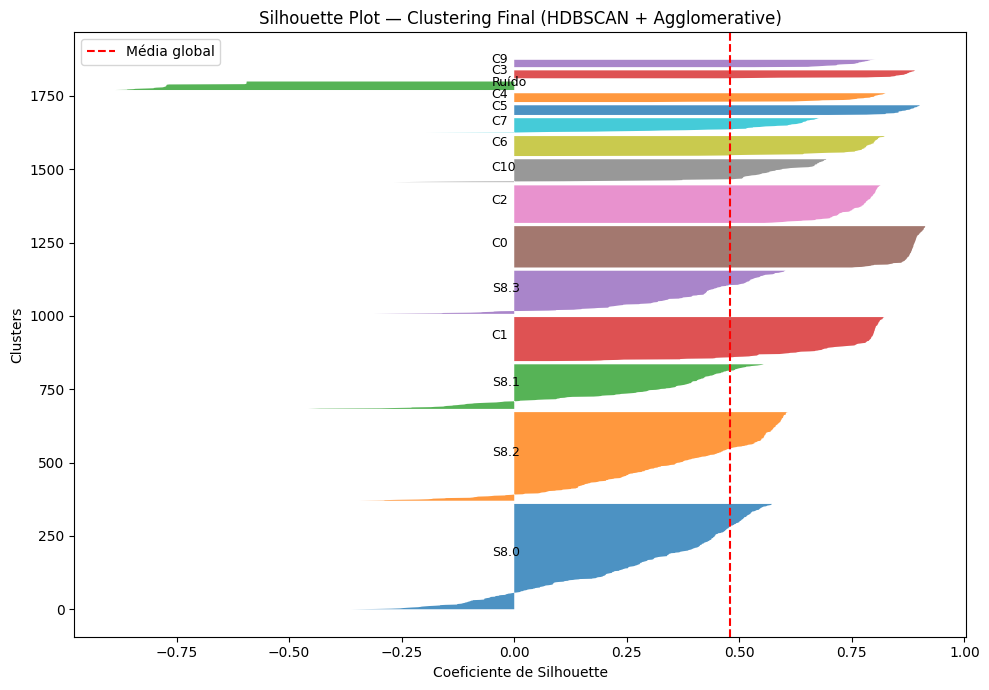
\includegraphics[width=0.95\textwidth]{sillhouette.png}
\caption{Silhouette Plot da clusterização final, combinando HDBSCAN global e clusterização aglomerativa para decomposição do supercluster. A linha tracejada indica a média global do coeficiente de Silhouette.}
\label{fig:silhouette-final}
\end{figure}

A presença de clusters com distribuições mais largas no eixo horizontal indica heterogeneidade interna, especialmente nos agrupamentos derivados do supercluster, o que é coerente com a natureza semântica contínua das rotas analisadas. Ainda assim, a predominância de valores positivos reforça a adequação da segmentação final obtida.

\subsection{Índice de Davies–Bouldin}

O índice de Davies–Bouldin (DBI) avalia a relação entre a dispersão interna dos clusters e a separação entre eles, assumindo valores não negativos, nos quais valores menores indicam melhor qualidade de clusterização. Essa métrica tende a penalizar agrupamentos com elevada variabilidade interna ou com centros próximos entre si.

No resultado final obtido, o índice de Davies–Bouldin apresentou valor igual a 1.1414. Esse valor indica uma separação moderada entre os clusters, refletindo o fato de que, embora os agrupamentos estejam globalmente bem definidos, alguns deles apresentam dispersão interna relativamente elevada ou proximidade espacial no espaço UMAP 3D. Esse comportamento é esperado, sobretudo nos clusters derivados da abertura hierárquica do supercluster, nos quais a granularidade semântica é maior e as fronteiras entre grupos são menos rígidas.

Assim, o valor observado do DBI não indica uma segmentação deficiente, mas sim a presença de clusters semanticamente relacionados, com transições graduais entre eles, característica típica de dados textuais representados em espaços semânticos contínuos. Esse resultado é coerente com a proposta exploratória do trabalho e com a interpretação qualitativa das projeções tridimensionais.

\subsection{Índice de Dunn}

O índice de Dunn mede a razão entre a menor distância inter-cluster e o maior diâmetro intra-cluster, sendo valores mais elevados indicativos de melhor separação relativa entre os agrupamentos. Essa métrica é particularmente sensível à presença de clusters extensos ou pouco compactos, uma vez que o denominador considera o maior espalhamento interno observado.

No presente experimento, o índice de Dunn calculado foi igual a 0.0037, um valor bastante baixo. Esse resultado indica que, embora exista separação entre os clusters, pelo menos um dos agrupamentos apresenta grande dispersão interna em relação à distância mínima observada entre clusters distintos. Tal comportamento é consistente com a presença do supercluster original e de seus subclusters derivados, que ocupam uma região extensa do espaço UMAP 3D e apresentam variações semânticas contínuas.

Dessa forma, o baixo valor do índice de Dunn não contradiz os resultados obtidos pelas demais métricas, mas reflete a natureza do conjunto de dados e da estratégia adotada. A segmentação foi projetada para preservar relações semânticas globais e permitir análises hierárquicas, e não para maximizar separações rígidas entre todos os agrupamentos, o que naturalmente impacta métricas sensíveis a dispersão extrema.

\subsection{Síntese Interpretativa}

A análise conjunta das métricas confirma que a clusterização final apresenta um equilíbrio adequado entre separação e expressividade semântica. O coeficiente de Silhouette indica boa coesão interna e separação média positiva entre os clusters, enquanto o índice de Davies–Bouldin aponta uma separação moderada, compatível com a existência de relações semânticas próximas entre determinados grupos. O índice de Dunn, por sua vez, evidencia a presença de clusters extensos e heterogêneos, resultado direto da decomposição controlada de um supercluster semanticamente amplo.

Em conjunto, esses resultados reforçam que a abordagem adotada — combinando redução de dimensionalidade não linear, clusterização baseada em densidade e decomposição hierárquica — é apropriada para a análise semântica de rotas Apache Camel. A estratégia privilegia interpretabilidade e exploração estrutural em detrimento de separações artificiais excessivamente rígidas, produzindo uma segmentação consistente com a complexidade intrínseca do domínio analisado.



% -------------------------------------------------
\section{Conclusão}

Este trabalho teve como objetivo aplicar técnicas de aprendizado não supervisionado para a análise e organização semântica de rotas Apache Camel, a partir de descrições textuais estruturadas e representações vetoriais obtidas por modelos de linguagem. O foco principal consistiu em investigar a capacidade dessas técnicas de revelar padrões estruturais, relações de similaridade e agrupamentos coerentes em um conjunto complexo e heterogêneo de rotas de integração.

Os resultados obtidos demonstram que a combinação de extração semântica baseada em modelos de linguagem, geração de embeddings textuais e técnicas de redução de dimensionalidade não linear constitui uma abordagem eficaz para a análise exploratória desse tipo de artefato de software. Em particular, observou-se que métodos lineares como o PCA são úteis para inspeção inicial, mas apresentam limitações na separação de estruturas semânticas mais complexas, enquanto técnicas não lineares como t-SNE e UMAP permitem capturar relações locais e globais de forma mais expressiva.

A utilização do UMAP em três dimensões, aliada a algoritmos de clusterização baseados em densidade, possibilitou identificar agrupamentos semanticamente relevantes e evidenciar a presença de um supercluster dominante. A decomposição desse supercluster por meio de clusterização hierárquica aglomerativa revelou subestruturas internas que não eram capturadas adequadamente por métodos baseados exclusivamente em densidade, resultando em uma segmentação mais interpretável e hierarquicamente organizada.

A avaliação quantitativa por meio das métricas de Silhouette, Davies–Bouldin e Dunn corroborou as análises visuais e estruturais realizadas ao longo do trabalho. Os valores obtidos refletem um equilíbrio entre separação e expressividade semântica, compatível com a natureza contínua dos dados textuais analisados e com a proposta exploratória da abordagem adotada. Em especial, a presença de clusters extensos e semanticamente variados explica as limitações observadas em métricas sensíveis à dispersão interna, sem comprometer a validade global da segmentação.

Como perspectiva de trabalhos futuros, destaca-se a necessidade de uma validação mais aprofundada da coesão semântica interna dos clusters obtidos. Uma possível estratégia consiste em empregar novamente modelos de linguagem para avaliar, de forma automática, a similaridade semântica entre as descrições das rotas pertencentes a um mesmo cluster, comparando-a com a similaridade entre rotas de clusters distintos. Alternativamente, pode-se formular essa validação como uma tarefa de classificação ou ranqueamento semântico, na qual o modelo avalia se elementos agrupados compartilham intenções arquiteturais e funcionais consistentes. Esse tipo de validação permitiria complementar as métricas geométricas utilizadas neste trabalho com uma avaliação semântica direta, reforçando a robustez e a interpretabilidade dos agrupamentos identificados.

Em síntese, o trabalho evidencia o potencial das técnicas de aprendizado não supervisionado, combinadas com modelos de linguagem, como ferramentas eficazes para a análise semântica de sistemas de integração, abrindo caminho para aplicações futuras em documentação automática, refatoração assistida e compreensão estrutural de arquiteturas complexas.


% -------------------------------------------------
\section*{Reprodutibilidade}

\begin{quote}
Código-fonte disponível em: 
\newline
\url{https://github.com/gilcesarf/imd3003-202502-projeto}
\end{quote}

As classes java bem como as descrições semanticas foram omitidas para preservar a confidencialidade do cliente. Entretanto, o arquivo com os embeddings gerados pode ser obtido no repositorio, de forma que os notebooks que executam os algoritmos podem ser executados.
O código-fonte das classes que processam os fontes Java e geram os embeddings, entretanto, estão disponíveis juntamente com os notebooks.
% -------------------------------------------------
\end{document}
